\documentclass{standalone}
\usepackage{tikz}
\usetikzlibrary{patterns, positioning}


\begin{document}
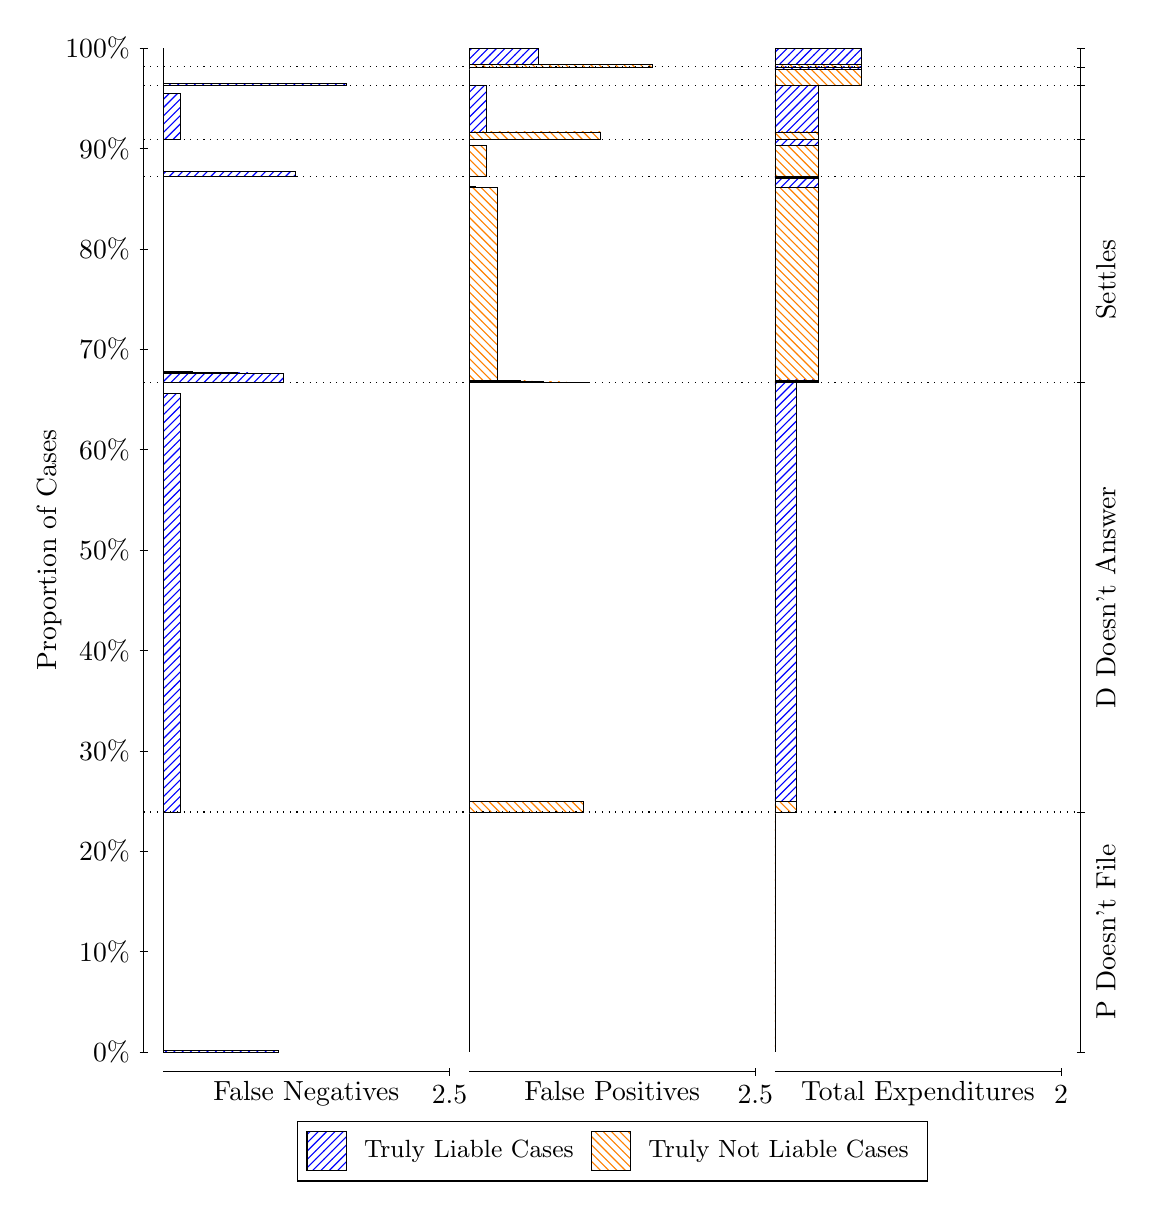
\begin{tikzpicture}
\draw[black, very thin] (1.5,1.75) -- (1.5,14.5);
\node[rotate=90, text=black, anchor=center] at (0.3, 8.125) {Proportion of Cases};
\draw[black, very thin] (1.45,1.75) -- (1.55,1.75);
\node[text=black, anchor=east] at (1.45, 1.75) {0\%};
\draw[black, very thin] (1.45,3.025) -- (1.55,3.025);
\node[text=black, anchor=east] at (1.45, 3.025) {10\%};
\draw[black, very thin] (1.45,4.3) -- (1.55,4.3);
\node[text=black, anchor=east] at (1.45, 4.3) {20\%};
\draw[black, very thin] (1.45,5.575) -- (1.55,5.575);
\node[text=black, anchor=east] at (1.45, 5.575) {30\%};
\draw[black, very thin] (1.45,6.85) -- (1.55,6.85);
\node[text=black, anchor=east] at (1.45, 6.85) {40\%};
\draw[black, very thin] (1.45,8.125) -- (1.55,8.125);
\node[text=black, anchor=east] at (1.45, 8.125) {50\%};
\draw[black, very thin] (1.45,9.4) -- (1.55,9.4);
\node[text=black, anchor=east] at (1.45, 9.4) {60\%};
\draw[black, very thin] (1.45,10.675) -- (1.55,10.675);
\node[text=black, anchor=east] at (1.45, 10.675) {70\%};
\draw[black, very thin] (1.45,11.95) -- (1.55,11.95);
\node[text=black, anchor=east] at (1.45, 11.95) {80\%};
\draw[black, very thin] (1.45,13.225) -- (1.55,13.225);
\node[text=black, anchor=east] at (1.45, 13.225) {90\%};
\draw[black, very thin] (1.45,14.5) -- (1.55,14.5);
\node[text=black, anchor=east] at (1.45, 14.5) {100\%};

\draw[black, very thin] (13.4,1.75) -- (13.4,14.5);
\draw[black, very thin] (13.35,1.75) -- (13.45,1.75);
\node[anchor=west] at (13.35, 1.75) {};
\draw[black, very thin] (13.35,4.7971) -- (13.45,4.7971);
\node[anchor=west] at (13.35, 4.7971) {};
\draw[black, very thin] (13.35,10.255) -- (13.45,10.255);
\node[anchor=west] at (13.35, 10.255) {};
\draw[black, very thin] (13.35,12.865) -- (13.45,12.865);
\node[anchor=west] at (13.35, 12.865) {};
\draw[black, very thin] (13.35,13.339) -- (13.45,13.339);
\node[anchor=west] at (13.35, 13.339) {};
\draw[black, very thin] (13.35,14.021) -- (13.45,14.021);
\node[anchor=west] at (13.35, 14.021) {};
\draw[black, very thin] (13.35,14.26) -- (13.45,14.26);
\node[anchor=west] at (13.35, 14.26) {};
\draw[black, very thin] (13.35,14.5) -- (13.45,14.5);
\node[anchor=west] at (13.35, 14.5) {};

\draw[black, very thin, pattern color=blue, pattern=north east lines] (1.75,1.75) rectangle (3.2033,1.7705);
\draw[black, very thin, pattern color=orange, pattern=north west lines] (1.75,1.7705) rectangle (1.75,4.7971);
\draw[black, very thin, pattern color=blue, pattern=north east lines] (1.75,4.7971) rectangle (1.968,10.116);
\draw[black, very thin, pattern color=orange, pattern=north west lines] (1.75,10.116) rectangle (1.75,10.255);
\draw[black, very thin, pattern color=blue, pattern=north east lines] (1.75,10.255) rectangle (3.276,10.369);
\draw[black, very thin, pattern color=blue, pattern=north east lines] (1.75,10.369) rectangle (3.1307,10.371);
\draw[black, very thin, pattern color=blue, pattern=north east lines] (1.75,10.371) rectangle (2.9853,10.372);
\draw[black, very thin, pattern color=blue, pattern=north east lines] (1.75,10.372) rectangle (2.84,10.374);
\draw[black, very thin, pattern color=blue, pattern=north east lines] (1.75,10.374) rectangle (2.6947,10.376);
\draw[black, very thin, pattern color=blue, pattern=north east lines] (1.75,10.376) rectangle (2.5493,10.377);
\draw[black, very thin, pattern color=blue, pattern=north east lines] (1.75,10.377) rectangle (2.404,10.378);
\draw[black, very thin, pattern color=blue, pattern=north east lines] (1.75,10.378) rectangle (2.2587,10.379);
\draw[black, very thin, pattern color=blue, pattern=north east lines] (1.75,10.379) rectangle (2.1133,10.392);
\draw[black, very thin, pattern color=orange, pattern=north west lines] (1.75,10.392) rectangle (1.75,12.865);
\draw[black, very thin, pattern color=blue, pattern=north east lines] (1.75,12.865) rectangle (3.4213,12.938);
\draw[black, very thin, pattern color=orange, pattern=north west lines] (1.75,12.938) rectangle (1.75,13.339);
\draw[black, very thin, pattern color=blue, pattern=north east lines] (1.75,13.339) rectangle (1.968,13.926);
\draw[black, very thin, pattern color=orange, pattern=north west lines] (1.75,13.926) rectangle (1.75,14.021);
\draw[black, very thin, pattern color=blue, pattern=north east lines] (1.75,14.021) rectangle (4.0753,14.054);
\draw[black, very thin, pattern color=orange, pattern=north west lines] (1.75,14.054) rectangle (1.75,14.26);
\draw[black, very thin, pattern color=orange, pattern=north west lines] (1.75,14.26) rectangle (1.75,14.294);
\draw[black, very thin, pattern color=blue, pattern=north east lines] (1.75,14.294) rectangle (1.75,14.5);
\draw[black, very thin, pattern color=orange, pattern=north west lines] (5.6333,1.75) rectangle (5.6333,4.7766);
\draw[black, very thin, pattern color=blue, pattern=north east lines] (5.6333,4.7766) rectangle (5.6333,4.7971);
\draw[black, very thin, pattern color=orange, pattern=north west lines] (5.6333,4.7971) rectangle (7.0867,4.9363);
\draw[black, very thin, pattern color=blue, pattern=north east lines] (5.6333,4.9363) rectangle (5.6333,10.255);
\draw[black, very thin, pattern color=orange, pattern=north west lines] (5.6333,10.255) rectangle (7.1593,10.256);
\draw[black, very thin, pattern color=orange, pattern=north west lines] (5.6333,10.256) rectangle (7.014,10.257);
\draw[black, very thin, pattern color=orange, pattern=north west lines] (5.6333,10.257) rectangle (6.8687,10.259);
\draw[black, very thin, pattern color=orange, pattern=north west lines] (5.6333,10.259) rectangle (6.7233,10.259);
\draw[black, very thin, pattern color=orange, pattern=north west lines] (5.6333,10.259) rectangle (6.578,10.267);
\draw[black, very thin, pattern color=orange, pattern=north west lines] (5.6333,10.267) rectangle (6.4327,10.267);
\draw[black, very thin, pattern color=orange, pattern=north west lines] (5.6333,10.267) rectangle (6.4327,10.273);
\draw[black, very thin, pattern color=orange, pattern=north west lines] (5.6333,10.273) rectangle (6.2873,10.279);
\draw[black, very thin, pattern color=orange, pattern=north west lines] (5.6333,10.279) rectangle (6.142,10.284);
\draw[black, very thin, pattern color=orange, pattern=north west lines] (5.6333,10.284) rectangle (5.9967,12.729);
\draw[black, very thin, pattern color=blue, pattern=north east lines] (5.6333,12.729) rectangle (5.706,12.741);
\draw[black, very thin, pattern color=blue, pattern=north east lines] (5.6333,12.741) rectangle (5.6333,12.865);
\draw[black, very thin, pattern color=orange, pattern=north west lines] (5.6333,12.865) rectangle (5.8513,13.266);
\draw[black, very thin, pattern color=blue, pattern=north east lines] (5.6333,13.266) rectangle (5.6333,13.339);
\draw[black, very thin, pattern color=orange, pattern=north west lines] (5.6333,13.339) rectangle (7.3047,13.434);
\draw[black, very thin, pattern color=blue, pattern=north east lines] (5.6333,13.434) rectangle (5.8513,14.021);
\draw[black, very thin, pattern color=orange, pattern=north west lines] (5.6333,14.021) rectangle (5.6333,14.227);
\draw[black, very thin, pattern color=blue, pattern=north east lines] (5.6333,14.227) rectangle (5.6333,14.26);
\draw[black, very thin, pattern color=orange, pattern=north west lines] (5.6333,14.26) rectangle (7.9587,14.294);
\draw[black, very thin, pattern color=blue, pattern=north east lines] (5.6333,14.294) rectangle (6.5053,14.5);
\draw[black, very thin, pattern color=orange, pattern=north west lines] (9.5167,1.75) rectangle (9.5167,4.7766);
\draw[black, very thin, pattern color=blue, pattern=north east lines] (9.5167,4.7766) rectangle (9.5167,4.7971);
\draw[black, very thin, pattern color=orange, pattern=north west lines] (9.5167,4.7971) rectangle (9.7892,4.9363);
\draw[black, very thin, pattern color=blue, pattern=north east lines] (9.5167,4.9363) rectangle (9.7892,10.255);
\draw[black, very thin, pattern color=orange, pattern=north west lines] (9.5167,10.255) rectangle (10.062,10.267);
\draw[black, very thin, pattern color=blue, pattern=north east lines] (9.5167,10.267) rectangle (10.062,10.285);
\draw[black, very thin, pattern color=orange, pattern=north west lines] (9.5167,10.285) rectangle (10.062,12.73);
\draw[black, very thin, pattern color=blue, pattern=north east lines] (9.5167,12.73) rectangle (10.062,12.845);
\draw[black, very thin, pattern color=orange, pattern=north west lines] (9.5167,12.845) rectangle (10.062,12.861);
\draw[black, very thin, pattern color=blue, pattern=north east lines] (9.5167,12.861) rectangle (10.062,12.865);
\draw[black, very thin, pattern color=orange, pattern=north west lines] (9.5167,12.865) rectangle (10.062,13.266);
\draw[black, very thin, pattern color=blue, pattern=north east lines] (9.5167,13.266) rectangle (10.062,13.339);
\draw[black, very thin, pattern color=orange, pattern=north west lines] (9.5167,13.339) rectangle (10.062,13.434);
\draw[black, very thin, pattern color=blue, pattern=north east lines] (9.5167,13.434) rectangle (10.062,14.021);
\draw[black, very thin, pattern color=orange, pattern=north west lines] (9.5167,14.021) rectangle (10.607,14.227);
\draw[black, very thin, pattern color=blue, pattern=north east lines] (9.5167,14.227) rectangle (10.607,14.26);
\draw[black, very thin, pattern color=orange, pattern=north west lines] (9.5167,14.26) rectangle (10.607,14.294);
\draw[black, very thin, pattern color=blue, pattern=north east lines] (9.5167,14.294) rectangle (10.607,14.5);
\draw[black, dotted] (1.5,4.7971) -- (13.4,4.7971);
\draw[black, dotted] (1.5,10.255) -- (13.4,10.255);
\draw[black, dotted] (1.5,12.865) -- (13.4,12.865);
\draw[black, dotted] (1.5,13.339) -- (13.4,13.339);
\draw[black, dotted] (1.5,14.021) -- (13.4,14.021);
\draw[black, dotted] (1.5,14.26) -- (13.4,14.26);
\draw[black, very thin] (1.75,1.5) -- (5.3833,1.5);
\node[text=black, anchor=north] at (3.5667, 1.5) {False Negatives};
\draw[black, very thin] (5.3833,1.45) -- (5.3833,1.55);
\node[text=black, anchor=north] at (5.3833, 1.45) {2.5};

\draw[black, very thin] (5.6333,1.5) -- (9.2667,1.5);
\node[text=black, anchor=north] at (7.45, 1.5) {False Positives};
\draw[black, very thin] (9.2667,1.45) -- (9.2667,1.55);
\node[text=black, anchor=north] at (9.2667, 1.45) {2.5};

\draw[black, very thin] (9.5167,1.5) -- (13.15,1.5);
\node[text=black, anchor=north] at (11.333, 1.5) {Total Expenditures};
\draw[black, very thin] (13.15,1.45) -- (13.15,1.55);
\node[text=black, anchor=north] at (13.15, 1.45) {2};

\node[text=black, centered, rotate=90] at (13.72, 3.2736) {P Doesn't File};
\node[text=black, centered, rotate=90] at (13.72, 7.5261) {D Doesn't Answer};
\node[text=black, centered, rotate=90] at (13.72, 11.56) {Settles};





\draw (7.449999999999999,1.5) node[draw=none] (baseCoordinate) {};
\begin{scope}[align=center]
        \matrix[scale=0.5, draw=black, below=0.5cm of baseCoordinate, nodes={draw}, column sep=0.1cm]{
            \node[rectangle, draw, minimum width=0.5cm, minimum height=0.5cm, pattern color=blue, pattern=north east lines] {}; &
            \node[draw=none, font=\small, text=black] (B) {Truly Liable Cases}; &
            \node[rectangle, draw, minimum width=0.5cm, minimum height=0.5cm, pattern color=orange, pattern=north west lines] {}; &
            \node[draw=none, font=\small, text=black] (B) {Truly Not Liable Cases}; \\
            };
\end{scope}

\end{tikzpicture}
\end{document}